\documentclass{article}
\usepackage{tikz}
\usepackage{mathtools}

\usetikzlibrary{shapes,arrows,matrix,fit}
% Diagrams styles
\tikzstyle{block} = [draw=black, rectangle, minimum height=2.5em, minimum width=2em]
\tikzstyle{sum} = [draw=black, circle]
\tikzstyle{gain} = [draw=black, regular polygon, regular polygon sides=3, regular polygon rotate=90, minimum height=2.5em, minimum width=2em]
\tikzstyle{input} = [coordinate]
\tikzstyle{output} = [coordinate]
\tikzstyle{pinstyle} = [pin edge={to-,thin,black}]

\begin{document}
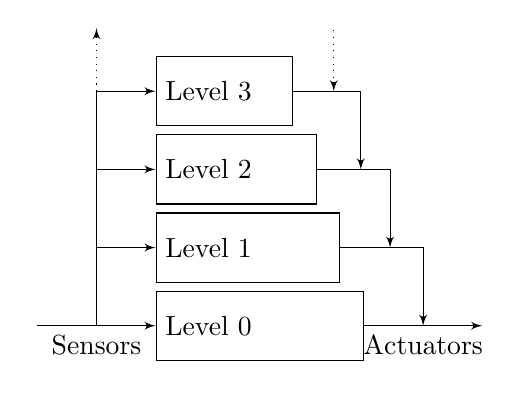
\begin{tikzpicture}[auto, node distance=2cm,>=latex']

	\matrix [draw=white, row sep=0.1cm, column sep=1.5cm] {	
	   	& \node [block, right, anchor=west, text width=1.5cm, minimum width=1.5cm] (levelD) {Level 3}; & \\
		& \node [block, right,anchor=west, text width=1.8cm, minimum width=1.8cm] (levelC) {Level 2}; & \\
	 	& \node [block, right,anchor=west, text width=2.1cm, minimum width=2.1cm] (levelB) {Level 1}; & \\
		\node [input,right] (input) {}; & \node [block,anchor=west, text width=2.4cm, right, minimum width=2.4cm] (levelA) {Level 0}; & \node[output](output){} ; \\
 	};

	\draw [->] (input) -- node[below](mid) {Sensors} (levelA);
	\draw [->] (mid) |- node {} (levelB);
	\draw [->] (mid) |- node(midU) {} (levelC);
	\draw [->] (mid) |- node (midUb)  {} (levelD);
	\draw [->] (levelA) -- node[below] (midA) {Actuators} (output);
	\draw [->] (levelB) -| node[pos=0.3] (midB) {} (midA);
	\draw [->] (levelC) -| node[pos=0.3] (midC) {} (midB.south);
	\draw [->] (levelD) -| node[pos=0.3] (midD) {} (midC.south);

	\draw [->,dotted] (midUb.south) -- node  {} ++(0,0.8);
	\draw [<-,dotted] (midD.south) -- node {} ++(0,0.8);
\end{tikzpicture}
\vspace{2cm}


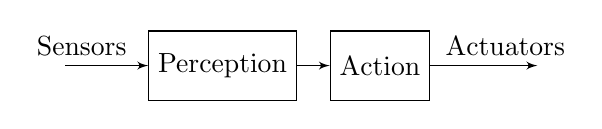
\begin{tikzpicture}[auto, node distance=2cm,>=latex']
	\node[input] (input) {};
	\node[block,right of=input] (perception) {Perception};
	\node[block,right of=perception] (action) {Action};
	\node[output, right of=action] (output) {};

	\draw[->] (input) -- node[pos=0.2] {Sensors} (perception);
	\draw[->] (perception) -- (action);
	\draw[->] (action) -- node[pos=0.7] {Actuators} (output);
\end{tikzpicture}

\vspace{2cm}


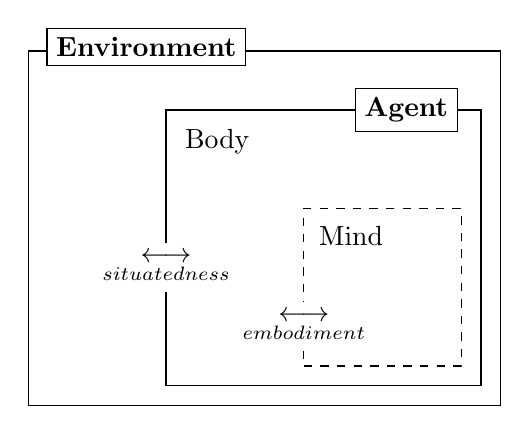
\begin{tikzpicture}[auto, node distance=1cm,>=latex']
	\node [rectangle, draw=black, minimum width=6cm,minimum height=4.5cm] (envir) {};
	\node [rectangle, draw=black, minimum width=4cm,minimum height=3.5cm] (body) at ++(0.75cm,-0.25cm) {};
	\node [rectangle, draw=black, dashed, minimum width=2cm,minimum height=2cm] (body) at ++(1.5cm,-0.75cm) {};
	\node [rectangle, fill=white] (situatedness) at ++(-1.25cm,-0.5cm) {$\underset{situatedness}{\longleftrightarrow}$};
	\node [rectangle, fill=white] (embodiment) at ++(.5cm,-1.25cm) {$\underset{embodiment}{\longleftrightarrow}$};
	\node [rectangle, fill=white, draw=black] at ++(-1.5cm,2.3cm) {\textbf{Environment}};
	\node [rectangle, fill=white, draw=black] at ++(1.8cm,1.5cm) {\textbf{Agent}};
	\node at(-0.6cm,1.1cm) {Body};
	\node at(1.1cm,-0.1cm) {Mind};
\end{tikzpicture}



\vspace{2cm}
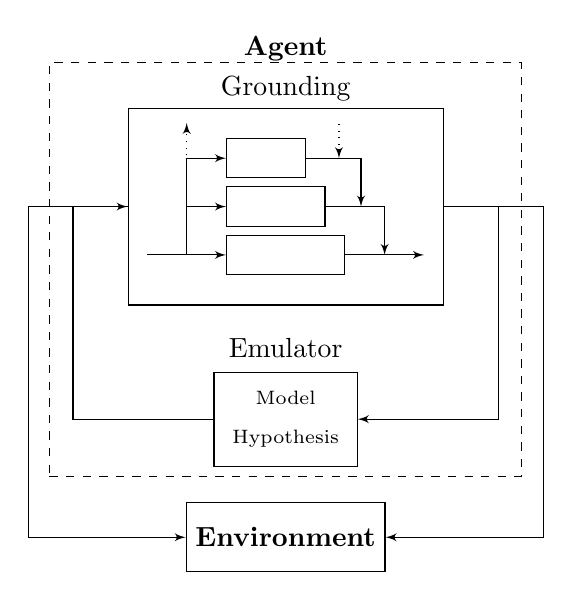
\begin{tikzpicture}[auto, node distance=2.7cm,>=latex']
	% EMULATION
	\matrix[draw=black, row sep=0.1cm, column sep=0.2cm] (emulator) {
	 \node {\scriptsize{Model}}; \\ 
	 \node {\scriptsize{Hypothesis}};  \\
	};
	\node[above of=emulator] at ++(0,-1.8cm) {Emulator};

	% GROUNDING
	\matrix [draw=black,minimum width=4cm, minimum height=2.5cm, row sep=0.1cm, column sep=1cm, above of=emulator] (grounding) at ++(0,0cm) {	
		& \node [block, right,anchor=west, minimum width=1cm ,minimum height=0.5cm] (levelC) {}; & \\
	 	& \node [block, right,anchor=west, minimum width=1.25cm ,minimum height=0.5cm] (levelB) {}; & \\
		\node [input,right] (input) {}; & \node [block,anchor=west, right, minimum width=1.5cm, minimum height=0.5cm] (levelA) {}; & \node[output](output){} ; \\
 	};
	\node[above of=grounding] at ++(0,1.5cm) {Grounding};

	% EMULATOR
	\node[block,below of=emulator] (environment) at ++(0,1.2cm) {\textbf{Environment}};


	\draw [->] (input) -- node[below](mid) {} (levelA);
	\draw [->] (mid) |- node (midK) {} (levelB);
	\draw [->] (mid) |- node(midU) {} (levelC);
	
	\draw [->] (levelA) -- node[below] (midA) {} (output);
	\draw [->] (levelB) -| node[pos=0.3] (midB) {} (midA);
	\draw [->] (levelC) -| node[pos=0.3] (midC) {} (midB.south);


	\draw [->,dotted] (mid) -- node  {} ++(0,1.8);
	\draw [<-,dotted] (midC.south) -- node {} ++(0,0.5);

	\node[right of=grounding] (gr) {};
	\node[left of=grounding] (gl) {};

	\draw [->] (emulator.west) -|  (gl.south) |- (grounding);
	\draw [<-] (emulator.east) -|  (gr.south) |- (grounding);

	\node[block,minimum width=6cm, minimum height=5.25cm,dashed] (agent) at ++(0,1.9cm) {};
	\node[above of=agent] at ++(0,2cm) {\textbf{Agent}};

	\draw [<-] (environment.east) -- ++(2cm,0) |- (grounding);
	\draw [<-] (environment.west) -- ++(-2cm,0) |- (grounding);

\end{tikzpicture}

\vspace{3cm}
  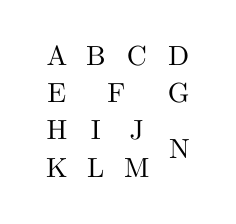
\begin{tikzpicture}
    \matrix (table) [%
      matrix of nodes,
      nodes in empty cells
    ] {%
      A & B & C & D \\
      E &   &   & G \\
      H & I & J &   \\
      K & L & M &   \\
   };
    \node[fit=(table-2-2)(table-2-3)]{F};
    \node[fit=(table-3-4)(table-4-4)]{N};
  \end{tikzpicture}
\end{document}